\documentclass{ximera}

%\addPrintStyle{..}


\begin{document}
	\author{Bart Lambregs}
	\xmtitle{Oefeningen schuine worp}{}
    \xmsource\xmuitleg

\begin{exercise} Leid een formule af die bij een schuine worp de dracht
(draagwijdte) geeft in functie van de beginsnelheid en de hoek
waaronder wordt geschoten.

\end{exercise}

\begin{exercise} Een projectiel wordt met een beginsnelheid van $350\rm\,m/s$
onder een hoek van $30^\circ$ met de horizontale afgeschoten.
\begin{enumerate}
\item Welke hoogte bereikt het projectiel?
\item Waar komt het projectiel op de grond?
\end{enumerate}
\footnote{$h=1561\rm\,m$, $d=10814\rm\,m$}

\end{exercise}

\begin{exercise} Een puntmassa wordt met een beginsnelheid van $40\rm\,m/s$
onder een hoek van $60^{\circ}$ opgeworpen.
\begin{enumerate}
\item Hoe groot is de snelheid in een punt op $35\rm\,m$ hoogte?
\item Hoe groot is de hoek, die de snelheid met de horizontale maakt in een punt
op $35\rm\,m$ hoogte boven de grond?
\item Waaraan is deze hoek gelijk als het voorwerp weer op dezelfde
hoogte is maar bij de dalende beweging?
\item Onder welke hoek treft het voorwerp de grond?
\end{enumerate}

\end{exercise}

\begin{exercise} Een obus wordt met een beginsnelheid $\vec{v}_0$ en onder een
hoek $\varphi$ weggeschoten. In het hoogste punt van zijn baan is:
\begin{enumerate}
\item $v_x=0\rm\,m/s$;
\item $v_x=h/t$;
\item $v_x=v_y$;
\item $v_x=v_0\cos{\varphi}$.
\end{enumerate}
\footnote{antwoord d}

\end{exercise}

\begin{exercise} Verschillende tennisballen worden met even grote snelheid maar
onder een verschillende hoek weggeschoten. De tennisbal die de
grootste dracht bereikt is deze die weggeschoten wordt onder een
hoek van:
\begin{enumerate}
\item 22,5$^\circ$;
\item 45,0$^\circ$;
\item 67,5$^\circ$;
\item 90,0$^\circ$.
\end{enumerate}
\footnote{antwoord b}

\end{exercise}

\begin{exercise} Twee raketten worden vanuit eenzelfde punt schuin
weggeschoten. Hun beginsnelheid is even groot en hun beginhoeken
zijn complementair ($\alpha+\beta=\frac{\pi}{2}$). Hebben deze
raketten dezelfde dracht?

\end{exercise}

\begin{exercise} Vanop de top van een kerktoren van $75,0\rm\,m$ hoog schiet
men een projectiel onder een hoek van $40^\circ$ met de horizontale
weg. De grootte van de beginsnelheid is $400\rm\,m/s$. Na hoeveel
tijd bereikt het projectiel de grond, en op welke afstand van de
voet van de toren? \footnote{$t=52,7\rm\,s$, $x=16151\rm\,m$}

\end{exercise}

\begin{exercise} Toon met een volledige opbouw aan dat de formule voor de
maximale hoogte bij de schuine worp wordt gegeven door:
\begin{displaymath}
h=\frac{v_0^2\sin^2{\varphi}}{2g}
\end{displaymath}

\end{exercise}

\begin{exercise} Een projectiel wordt afgevuurd met een beginsnelheid
$\vec{v}_0$ die een hoek $\varphi$ maakt met de horizontale
\mbox{$x$-as}.
% \newline
In de veronderstelling dat de luchtweerstand verwaarloosbaar is, dan
ziet het verloop van de horizontale snelheidscomponente $v_x$ als
functie van de tijd er als volgt uit:
\begin{image}
% \begin{flushright}
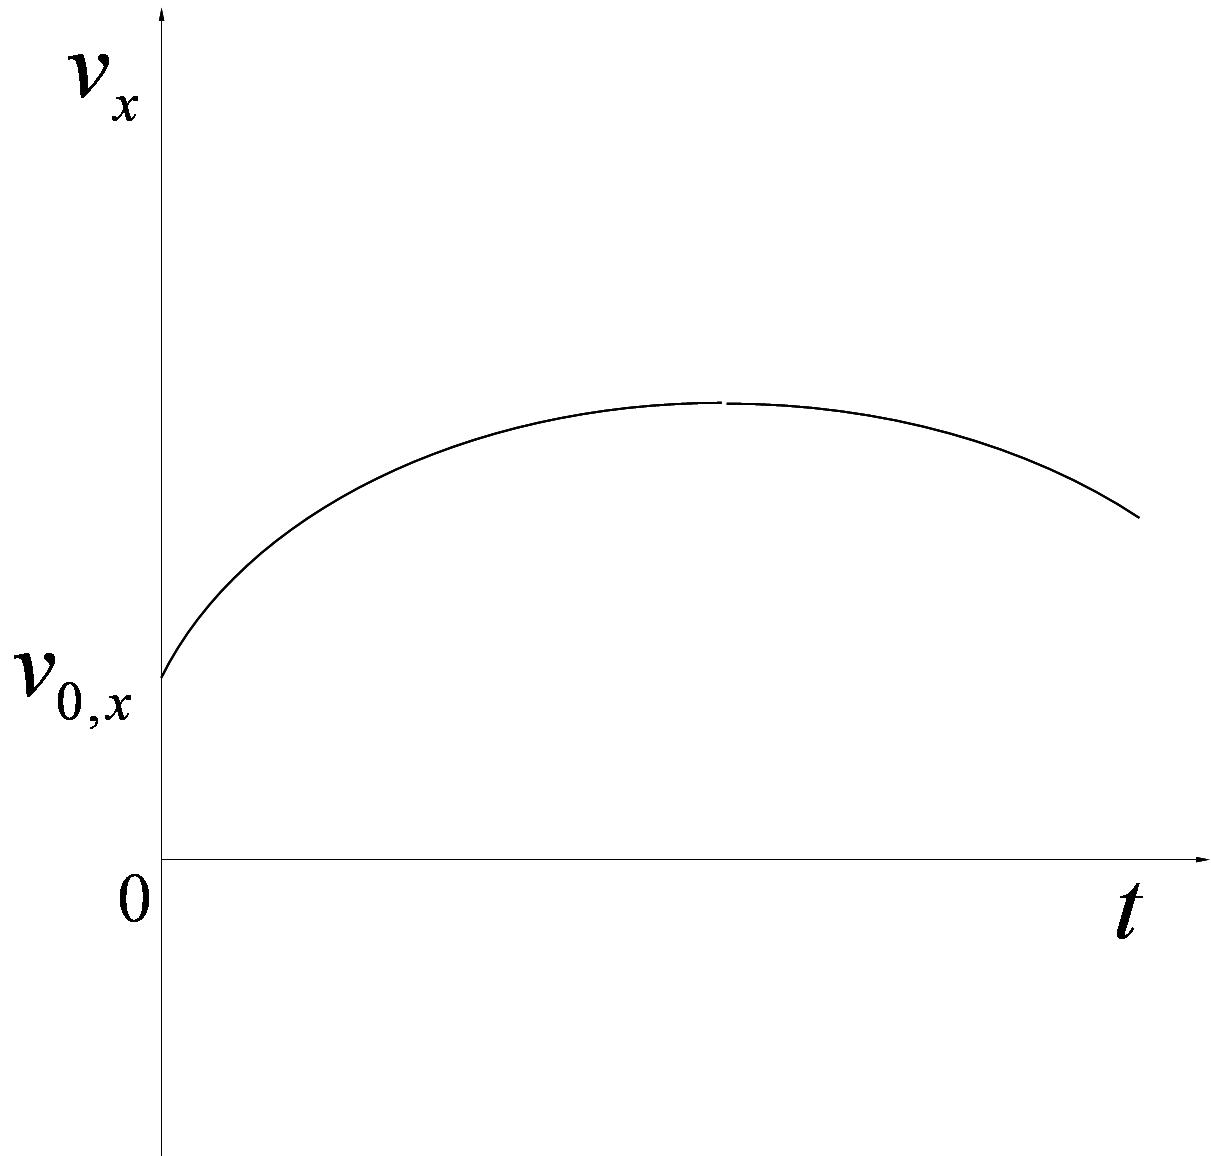
\includegraphics[width=0.22\textwidth, angle=0]{horiz_snelheidscomp_a}
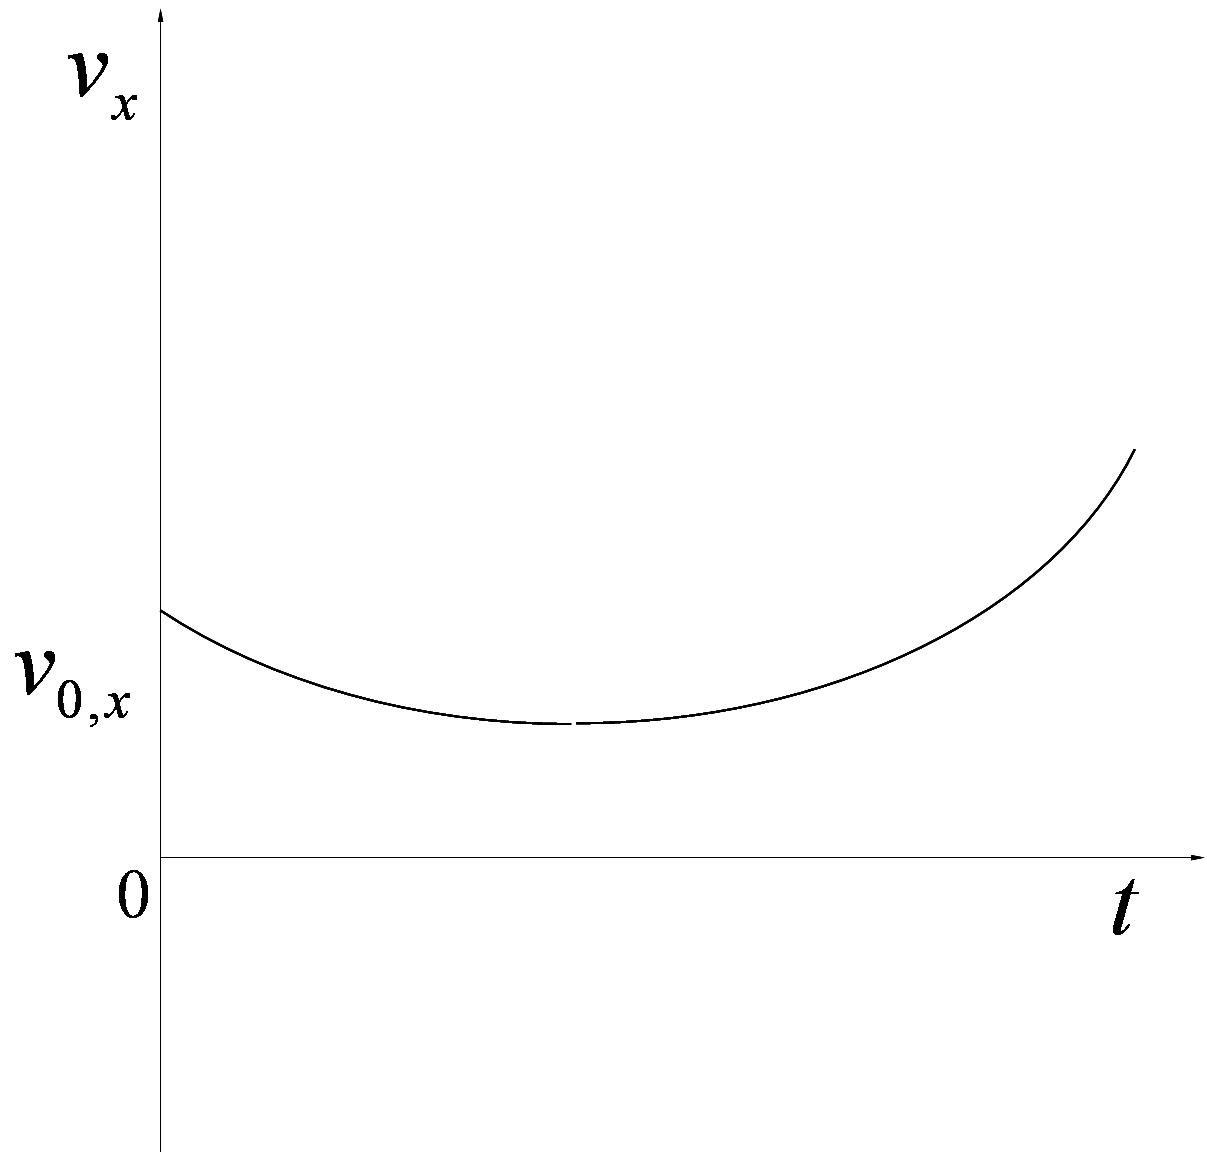
\includegraphics[width=0.22\textwidth, angle=0]{horiz_snelheidscomp_b}
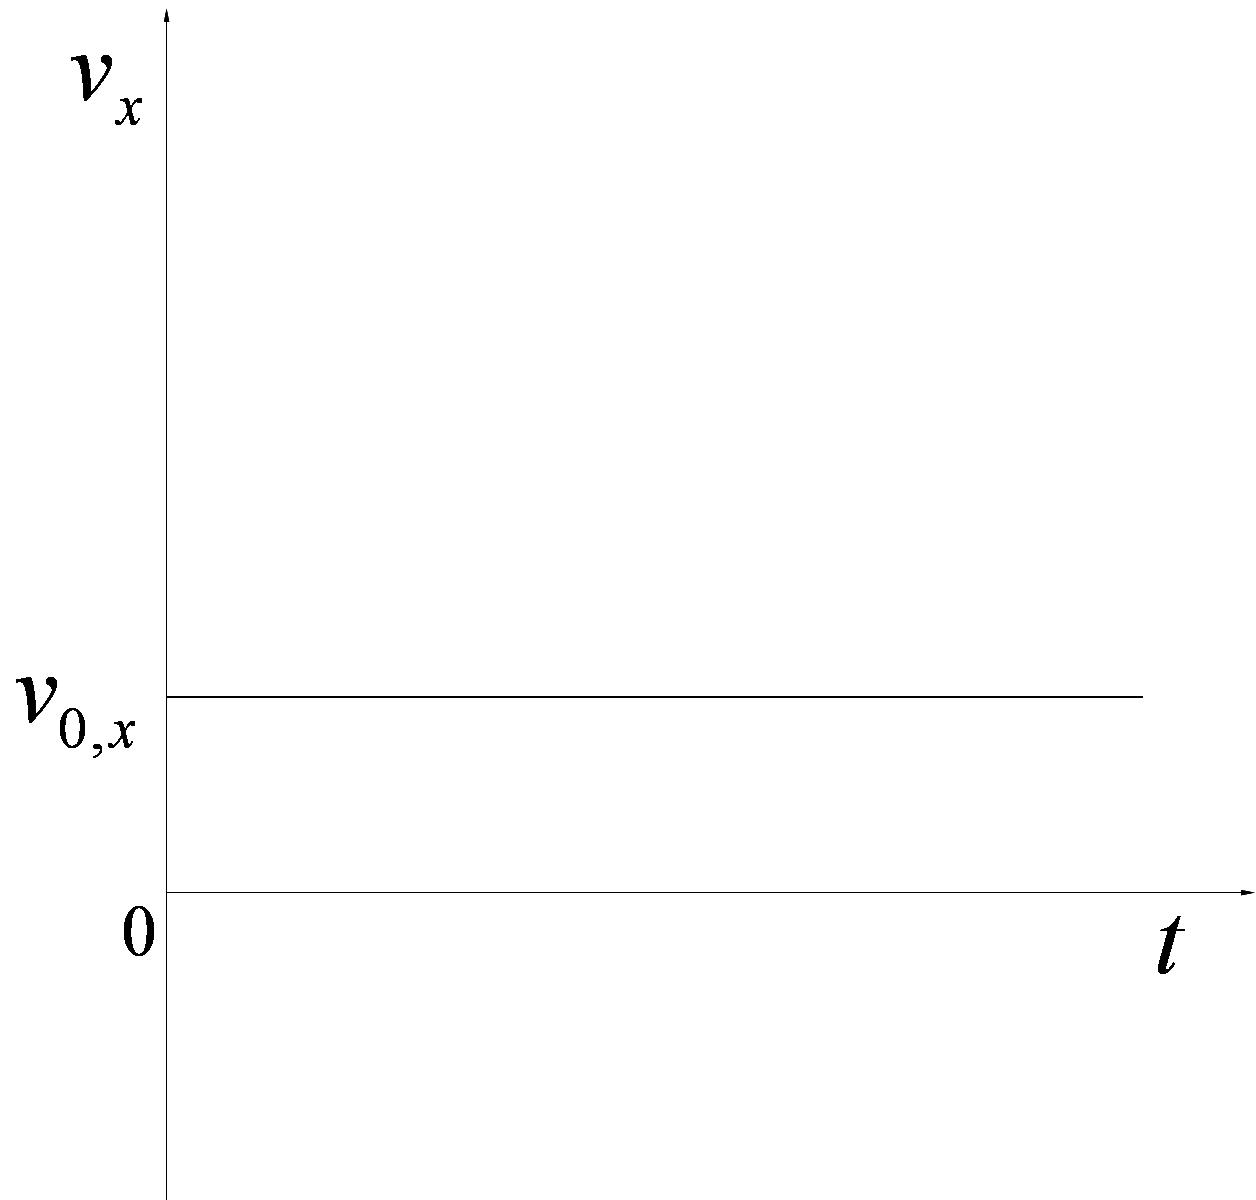
\includegraphics[width=0.22\textwidth, angle=0]{horiz_snelheidscomp_c}
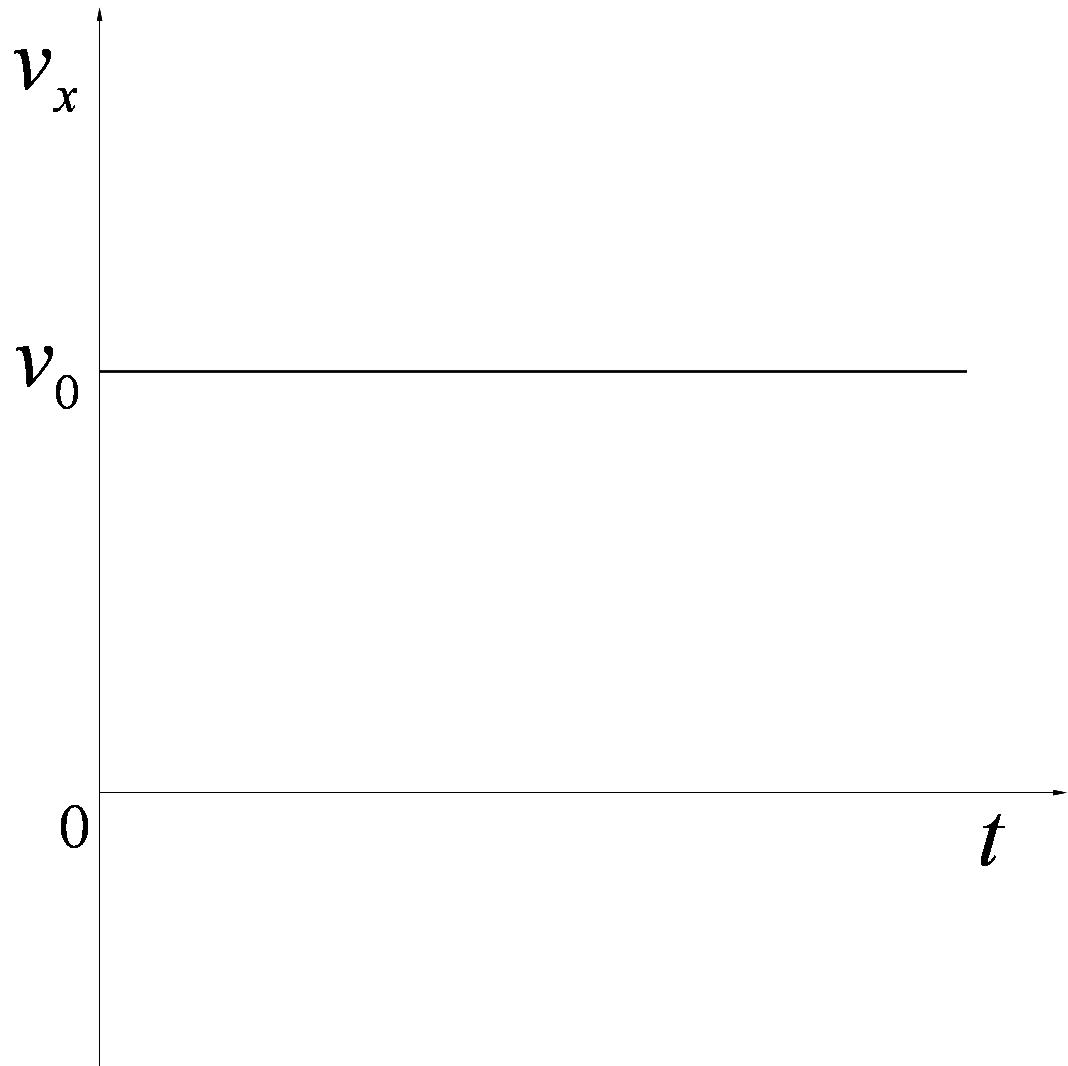
\includegraphics[width=0.22\textwidth, angle=0]{horiz_snelheidscomp_d}
% \end{flushright}
\end{image}

\end{exercise}

\begin{exercise} Onderstaande figuur stelt de baan voor van
een kogel die op het ogenblik \mbox{$t=0$~s} afgeschoten wordt
vanuit de oorsprong. De aangeduide punten geven om de \mbox{100 ms}
de plaats van de kogel aan.
\begin{image}
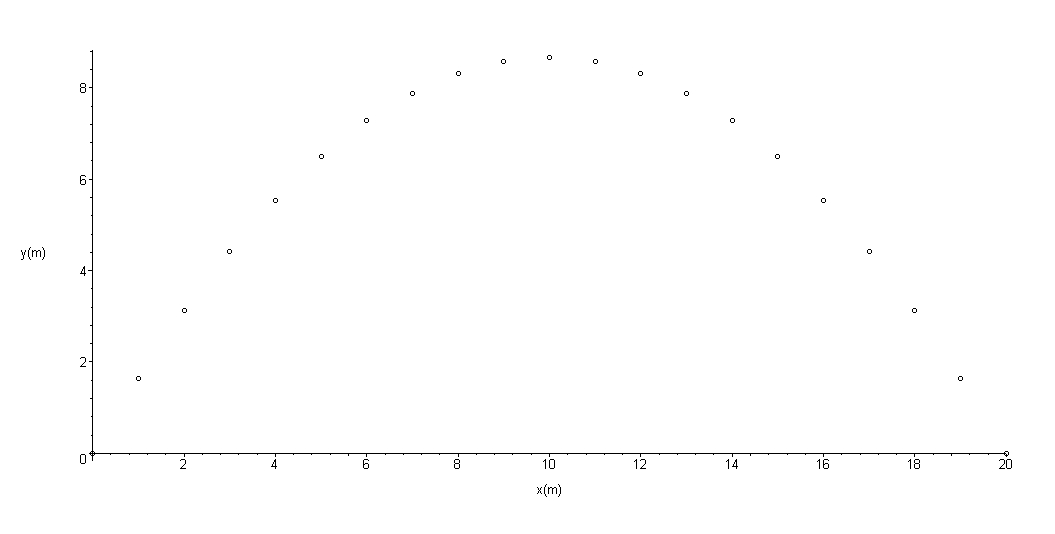
\includegraphics[width=0.7\textwidth]{horiz_snelheidscomp}
\end{image}


De horizontale snelheidscomponent van de kogel is gelijk aan?
\begin{enumerate}
\item 5 m/s
\item 10 m/s
\item 15 m/s
\item 20 m/s
\end{enumerate}

\end{exercise}

\begin{exercise} Nadat de kerstman zijn speelgoed op de
gebruikelijke manier geleverd heeft, wil hij zich ook eens amuseren
en glijdt langs het beijzeld dak naar beneden. Hij vertrekt vanuit
rust op de top van het dak dat $8,2~\rm m$ lang is met een
versnelling van $5,0~\rm m/s^2$. De rand van het dak bevindt zich
$3,0~\rm m$ boven de grond die met een pak sneeuw bedekt is.
\begin{image}
% \begin{center}
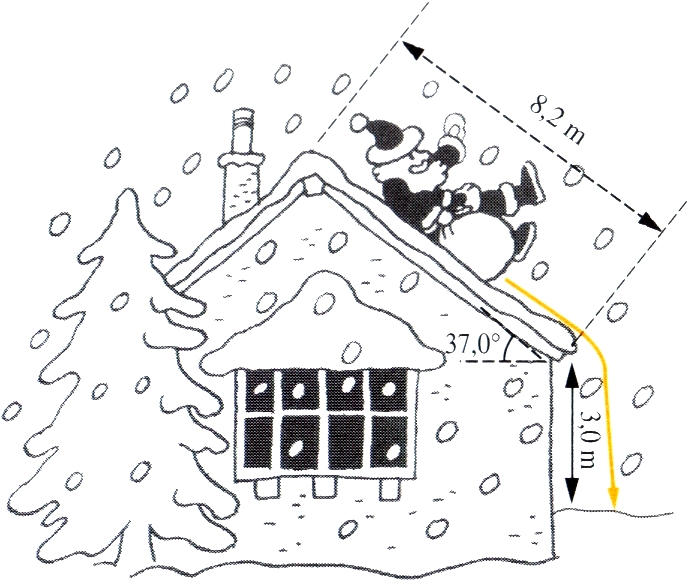
\includegraphics[width=0.55\textwidth]{kerstman}
% \end{center}
\end{image}
\begin{enumerate}
\item Hoe groot is de snelheid van de kerstman waarmee hij van het
dak vliegt?
\item Hoe groot is de afstand $d$ tussen het huis en het punt waar
hij in de sneeuw terecht komt?\footnote{De baanvergelijking voor de
schuine worp:
\[
y=x\tan\varphi-\frac{g}{2v_0^2\cos^2\varphi}x^2
\]}
\end{enumerate}

\end{exercise}

\end{document}
